\documentclass{article}

\input{../homework.sty}

\title{Homework 1}
\author{Austin Gill}

\begin{document}
\maketitle

\section*{The Fibonacci Bug}
    It's really hard to parallelize when the sequence definition is a recurrence relation. There is a strong dependence of the $n$th term on the $(n-1)$th and $(n-2)$th terms. This doesn't parallelize because there is an inherent order requirement, essentially forcing a sequential execution.

    Now, there \textit{is} a way to make the code parallel.

   \begin{quote}
       Given a homogeneous linear recurrence relation with constant coefficients (a discrete case of a differential equation)

       \[ a_0 x(n) + a_1 x(n - 1) + a_2 x(n - 2) + \cdots + a_m x(n - m) = 0 \]

       We assume a solution of the form $x(n) = C\lambda^n$ and substitute:

       \[ a_0 C\lambda^n + a_1 C \lambda^{n - 1} + \cdots + a_m C \lambda^{n - m} = 0 \]
       \[ a_0 \lambda^n + a_1 \lambda^{n - 1} + \cdots + a_m \lambda^{n - m} = 0 \]
       \[ \lambda^{n - m} \underbrace{( a_0 \lambda^m + a_1 \lambda^{m - 1} + \cdots + a_m \lambda^0 )}_{\text{Characteristic equation with roots as solutions}} = 0 \]

       In the case of no repeated roots, we have

       \[ x(n) = c_1 \lambda_1^n + c_2 \lambda_2^n + \cdots + c_m \lambda_m^n \]

       where each $\lambda_i$ is an eigenvalue, and each $c_i$ is found from the initial conditions. We say that the dominant eigenvalue is the eigenvalue with the greatest absolute value.

       \[ \lambda_d = \max_i\{ \vert \lambda_i \vert \} \]
   \end{quote}

   Now returning to the Fibonacci sequence, a second order recurrence relation (requiring two initial conditions to solve)

   \[ x(n) - x(n - 1) - x(n - 2) = 0 \]
   \[ x(n) = C\lambda^n \rightsquigarrow C\lambda^n - C \lambda^{n - 1} - C\lambda^{n - 2} = 0 \]

   Factoring out $C\lambda^{n - 2}$ gives us the characteristic equation

   \[ \lambda^2 - \lambda - 1 = 0 \]

   which has roots

   \[ \lambda = \frac{1 \pm \sqrt{1 - 4(-1)(1)}}{2} = \frac{1 \pm \sqrt{5}}{2} \]

   where $\frac{1 + \sqrt{5}}{2}$, a.k.a., the golden ratio $\phi$, is the dominant eigenvalue. So then the recurrence relation has the solution

   \[ x(n) = c_1 {\left(\frac{1 + \sqrt{5}}{2}\right)}^n + c_2 {\left(\frac{1 - \sqrt{5}}{2}\right)}^n \]

   where we solve for $c_1$ and $c_2$ using the initial conditions $x(0) = 1$ and $x(1) = 1$.

   \[ x(0) = 1 = c_1 + c_2 \]
   \[ x(1) = 1 = c_1 \left( \frac{1 + \sqrt{5}}{2} \right) + c_2 \left( \frac{1 - \sqrt{5}}{2} \right) \]

   which gives $c_1 = \frac{1}{\sqrt{5}}$ and $c_2 = - \frac{1}{\sqrt{5}}$.

   So all together then, the closed form solution of the homogeneous Fibonacci linear recurrence relation is

   \[x(n) = \frac{1}{\sqrt{5}} \left( {\left( \frac{1 + \sqrt{5}}{2} \right)}^n - {\left( \frac{1 - \sqrt{5}}{2} \right)}^n \right)\]

   Note that this closed form has no history dependence, so it \textit{will} parallelize quite nicely, ignoring the increased number of floating point operations required to compute each $x(n)$ value.


\section{}
    \begin{quote}
        Recall that OpenMP creates private variables for reduction variables, and these private variables are initialized to the identity element for the reduction operator. For example, if the operator is addition, the private variables are initialized to 0, while if the operator is multiplication, the private variables are initialized to 1.

        What are the identity values for these operators: \mintinline{c}{&&}, \mintinline{c}{||}, \mintinline{c}{|}, and \mintinline{c}{^}?
    \end{quote}

    The mathematical identity for $\land$ is $T$, because $x \land T \equiv x$, thus the identity for the \mintinline{c}{&&} operator is \mintinline{cpp}{true}. Similarly, the identity for the \mintinline{c}{||} operator is \mintinline{cpp}{false}. The identities for the bitwise operations \mintinline{c}{|} and \mintinline{c}{^} are both \mintinline{c}{0x0}.

\section{}
    \begin{quote}
        Suppose OpenMP did not have the \mintinline{c}{reduction} clause. Show how to implement an \textit{efficient} parallel reduction by adding a private variable and using the \mintinline{c}{critical} pragma.
    \end{quote}

    Consider the following three solutions.

    \begin{enumerate}
        \item Normal reduction: \begin{minted}{c}
            size_t sum1 = 0;
            #pragma omp parallel for num_threads( 8 ) reduction(+:sum1)
            for( size_t i = 0; i < n; ++i )
            {
                sum1 += i;
            }
        \end{minted}

        \item Naive reduction, which is even worse than sequential: \begin{minted}{c}
            size_t sum2 = 0;
            size_t local_sum = 0;
            #pragma omp parallel for num_threads( 8 ) private( local_sum )
            for( size_t i = 0; i < n; ++i )
            {
                local_sum = i;

                // This is wrong. It's essentially sequential with a lot of overhead.
                #pragma omp critical
                sum2 += local_sum;
            }
        \end{minted}

        \item Better reduction, which performs slightly \textit{better} than using \mintinline{c}{reduction}: \begin{minted}{c}
            size_t sum3 = 0;
            #pragma omp parallel num_threads( 8 )
            {
                size_t local_sum = 0;
                #pragma omp for
                for(size_t i = 0; i < n; ++i )
                {
                    local_sum += i;
                }

                #pragma omp critical
                sum3 += local_sum;
            }
        \end{minted}
    \end{enumerate}

    All together, with timing code and \mintinline{c}{n = 1000000} we get the following results.

    \begin{minted}{text}
        reduced sum:  499999500000
        elapsed time: 13.664000ms
        naive sum:    499999500000
        elapsed time: 76.582000ms
        critical sum: 499999500000
        elapsed time: 0.291000ms
    \end{minted}

\section{}
    \begin{quote}
        For each of the following code segments, use OpenMP pragmas to make the loop parallel, or explain why the code segment is not suitable for parallel execution.

        % \begin{enumerate}
        %     \item \begin{minted}{c}
        %         for(i = 0; i < (int) sqrt(x); i++)
        %         {
        %             a[i] = 2.3 * i;
        %             if(i < 10)
        %                 b[i] = a[i];
        %         }
        %     \end{minted}

        %     \item \begin{minted}{c}
        %         flag = 0;
        %         for(i = 0; i < n && !flag; i++)
        %         {
        %             a[i] = 2.3 * i;
        %             if(a[i] < b[i])
        %                 flag = 1;
        %         }
        %     \end{minted}

        %     \item \begin{minted}{c}
        %         for(i = 0; i < n; i++)
        %         {
        %             a[i] = foo(i);
        %         }
        %     \end{minted}

        %     \item \begin{minted}{c}
        %         for(i = 0; i < n; i++)
        %         {
        %             a[i] = foo(i);
        %             if(a[i] > b[i])
        %                 a[i] = b[i];
        %         }
        %     \end{minted}

        %     \item \begin{minted}{c}
        %         for(i = 0; i < n; i++)
        %         {
        %             a[i] = foo(i);
        %             if(a[i] < b[i])
        %                 break;
        %         }
        %     \end{minted}

        %     \item \begin{minted}{c}
        %         dotp = 0;
        %         for(i = 0; i < n; i++)
        %         {
        %             dotp += a[i] * b[i];
        %         }
        %     \end{minted}

        %     \item \begin{minted}{c}
        %         for(i = k; i < 2 * k; i++)
        %         {
        %             a[i] = a[i] + a[i-k];
        %         }
        %     \end{minted}

        %     \item \begin{minted}{c}
        %         for(i = k; i < n; i++)
        %         {
        %             a[i] = b * a[i - k];
        %         }
        %     \end{minted}
        % \end{enumerate}
    \end{quote}

    \begin{enumerate}
        \item \begin{minted}{c}
            #pragma omp parallel for num_threads( 8 )
            for(i = 0; i < (int) sqrt(x); i++)
            {
                a[i] = 2.3 * i;
                if(i < 10)
                    b[i] = a[i];
            }
        \end{minted}

        \item Cannot use OpenMP to parallelize because the loop is not fixed in size.
        \begin{minted}{text}
            prob3.c: In function ‘main’:
            prob3.c:50:23: error: invalid controlling predicate
                 for(size_t i = 0; i < 9 && !flag; i++)
                                   ^
        \end{minted}

        \item \begin{minted}{c}
            #pragma omp parallel for num_threads( 8 )
            for(i = 0; i < n; i++)
            {
                a[i] = foo(i);
            }
        \end{minted}

        \item \begin{minted}{c}
            #pragma omp parallel for num_threads( 8 )
            for(i = 0; i < n; i++)
            {
                a[i] = foo(i);
                if(a[i] > b[i])
                    a[i] = b[i];
            }
        \end{minted}

        \item Cannot use OpenMP to parallelize because the loop is not fixed in size.

        \item \begin{minted}{c}
            dotp = 0;
            #pragma omp parallel for num_threads( 8 ) reduce(+: dotp)
            for(i = 0; i < n; i++)
            {
                dotp += a[i] * b[i];
            }
        \end{minted}

        \item Cannot parallelize because you cannot easily guarantee \mintinline{c}{a[i - k]} will be properly computed \textit{before} \mintinline{c}{a[i]}, as in the Fibonacci sequence assigned over the weekend. Since \mintinline{c}{k} is fixed, there might be a way to force the loop division over the threads to play nicely, but this would be too much work for too little reward, and would have the added benefit of confusing the hell out of anyone who tried to understand your code.

        \item Same as above.
    \end{enumerate}

\section{}
    \begin{quote}
        Given a task that can be divided into $m$ subtasks, each requiring one unit of time, how much time is needed for an $m$-stage pipeline to process $n$ tasks?
    \end{quote}

    Assuming that each task is broken into $m$ strictly ordered sequential subtasks, we have a few choices. You can use $n$ workers, each performing the full task. Then the amount of time will be on the order of however long it takes to complete a single task. However, this doesn't scale well; we normally have more tasks than each task has subtasks.

    We can use $m$ workers, each performing a single sub task in an offset manner so that worker 1 completes subtask 1 for task 1 and begins subtask 1 for task 2 as worker 2 begins subtask 2 for task 1 and so on. This will complete in $\sim \mathcal O(n)$ time.

    We can use $jm$ workers and have $j$ copies of the pipeline running side-by-side. This also completes in $\sim \mathcal O(n)$ time.

\section{}
    \begin{quote}
        If the address of the nodes in a hypercube has $n$ bits, at most how many nodes can there be, and how many edges does each node have?

        Give an algorithm that routes a message from node $u$ to node $v$ in this $k$-node hypercube in no more than $\log k$ steps.
    \end{quote}

    There will be $2^n$ nodes with $n$ edges per node.

    \begin{minted}{python}
        intermediate_address = u
        # Iterate over the bits of the address.
        for i, u_b, v_b in enumerate(zip(u, v)):
            # Flip the differing bits of the src address one-by-one
            if u_b != v_b:
                intermediate_address[i] = v_b
                mailman.send(msg, intermediate_address)
    \end{minted}

\section{}
    \begin{quote}
        Research the \textit{shuffle-exchange} network topology. Draw the network with 16 processor nodes (numbering each node in binary, showing shuffle and exchange links). If there are $k$ bits in the address, how many nodes are there? With $n$ nodes, what is the diameter and bisection width of the network? How many edges per node are there?
    \end{quote}

    In a shuffle-exchange network with $2^n$ nodes addressed with $n$ bit addresses, there is a directed edge between two nodes if one of the following holds.

    \begin{description}
        \item[shuffle] One address is a 1-bit cyclic left shift of the other. This forms a directed shuffle edge.
        \item[exchange] The addresses differ only in the last bit. This forms a directed exchange edge.
    \end{description}

    Each node has two outgoing edges and two incoming edges, one each of shuffle and exchange. The network has a bisection width of $2^{n - 1}$ and a diameter of $2n - 1$.

    So the 4 node network shown in~\autoref{fig:shuffle4}.

    \begin{figure}
        \centering
        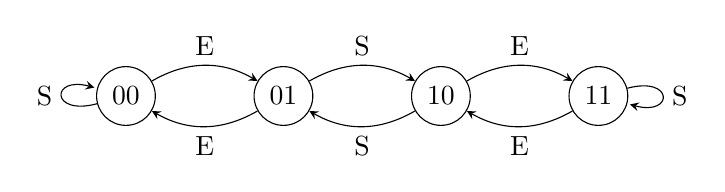
\begin{tikzpicture}[>=stealth, node distance=2cm]
            \tikzset{vertex/.style = {shape=circle, draw, minimum size=1em}}

            \node[vertex] (00) {$00$};
            \node[vertex, right of=00] (01) {$01$};
            \node[vertex, right of=01] (10) {$10$};
            \node[vertex, right of=10] (11) {$11$};

            \draw[->, loop left] (00) edge node[left]{S} (00);
            \draw[->, loop right] (11) edge node[right]{S} (11);

            \draw[->, bend left] (01) edge node[above]{S} (10);
            \draw[->, bend left] (10) edge node[below]{S} (01);

            \draw[->, bend left] (00) edge node[above]{E} (01);
            \draw[->, bend left] (01) edge node[below]{E} (00);

            \draw[->, bend left] (10) edge node[above]{E} (11);
            \draw[->, bend left] (11) edge node[below]{E} (10);
        \end{tikzpicture}
        \caption{A 4 node (2 bit) shuffle-exchange network}\label{fig:shuffle4}
    \end{figure}

    Now consider the following Python script \inputminted{python}{prob6.py}

    which produces, in part the network shown in~\autoref{fig:shuffle16}.

    \afterpage{%
    \thispagestyle{empty}
    \newgeometry{margin=0cm}
    \begin{figure}
        \centering
        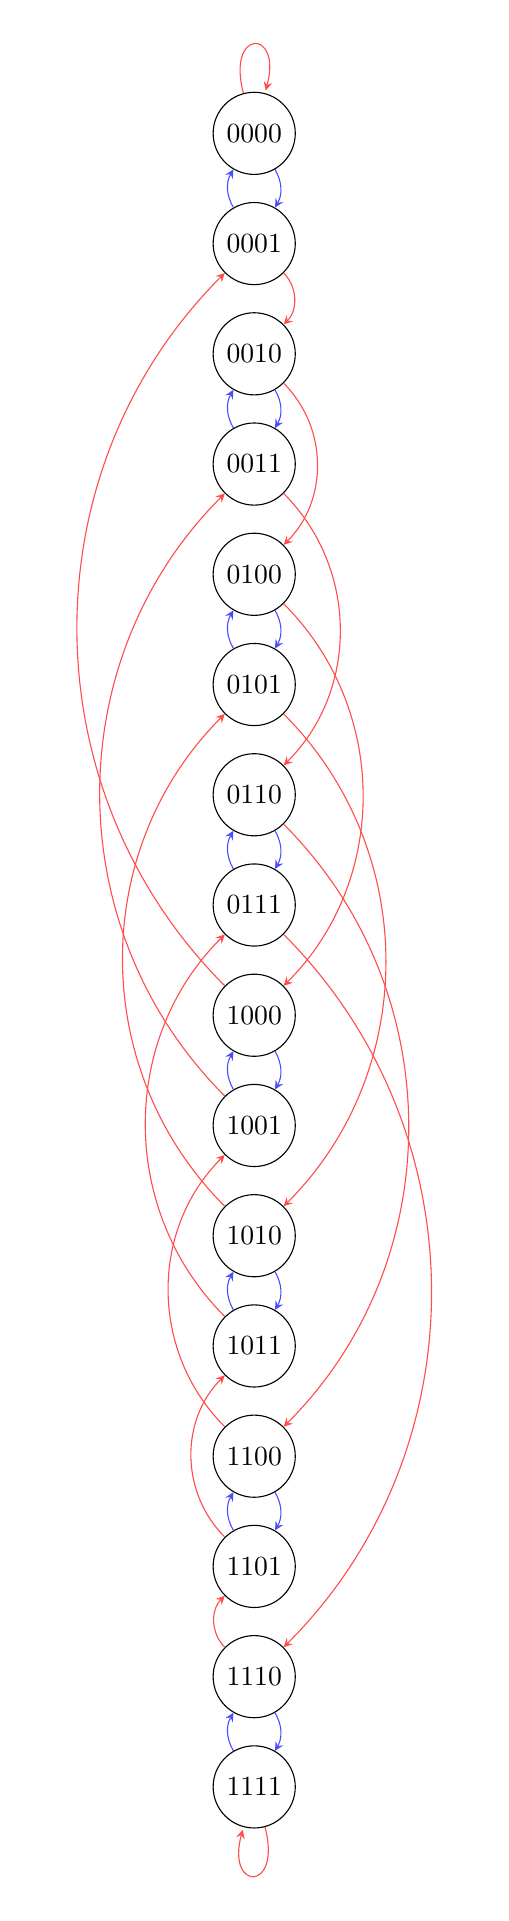
\begin{tikzpicture}[>=stealth, node distance=1.4cm]
            \tikzset{vertex/.style = {shape=circle, draw, minimum size=1em}}

            \node[vertex] (0000) {$0000$};
            \node[vertex, below of=0000] (0001) {$0001$};
            \node[vertex, below of=0001] (0010) {$0010$};
            \node[vertex, below of=0010] (0011) {$0011$};

            \node[vertex, below of=0011] (0100) {$0100$};
            \node[vertex, below of=0100] (0101) {$0101$};
            \node[vertex, below of=0101] (0110) {$0110$};
            \node[vertex, below of=0110] (0111) {$0111$};

            \node[vertex, below of=0111] (1000) {$1000$};
            \node[vertex, below of=1000] (1001) {$1001$};
            \node[vertex, below of=1001] (1010) {$1010$};
            \node[vertex, below of=1010] (1011) {$1011$};

            \node[vertex, below of=1011] (1100) {$1100$};
            \node[vertex, below of=1100] (1101) {$1101$};
            \node[vertex, below of=1101] (1110) {$1110$};
            \node[vertex, below of=1110] (1111) {$1111$};

            \draw[->, color=blue!70, bend left] (0000) edge (0001);
            \draw[->, color=blue!70, bend left] (0001) edge (0000);
            \draw[->, color=blue!70, bend left] (0010) edge (0011);
            \draw[->, color=blue!70, bend left] (0011) edge (0010);
            \draw[->, color=blue!70, bend left] (0100) edge (0101);
            \draw[->, color=blue!70, bend left] (0101) edge (0100);
            \draw[->, color=blue!70, bend left] (0110) edge (0111);
            \draw[->, color=blue!70, bend left] (0111) edge (0110);
            \draw[->, color=blue!70, bend left] (1000) edge (1001);
            \draw[->, color=blue!70, bend left] (1001) edge (1000);
            \draw[->, color=blue!70, bend left] (1010) edge (1011);
            \draw[->, color=blue!70, bend left] (1011) edge (1010);
            \draw[->, color=blue!70, bend left] (1100) edge (1101);
            \draw[->, color=blue!70, bend left] (1101) edge (1100);
            \draw[->, color=blue!70, bend left] (1110) edge (1111);
            \draw[->, color=blue!70, bend left] (1111) edge (1110);

            \draw[->, color=red!70, loop above] (0000) edge (0000);
            \draw[->, color=red!70, bend left=45] (0001) edge (0010);
            \draw[->, color=red!70, bend left=45] (0010) edge (0100);
            \draw[->, color=red!70, bend left=45] (0011) edge (0110);
            \draw[->, color=red!70, bend left=45] (0100) edge (1000);
            \draw[->, color=red!70, bend left=45] (0101) edge (1010);
            \draw[->, color=red!70, bend left=45] (0110) edge (1100);
            \draw[->, color=red!70, bend left=45] (0111) edge (1110);
            \draw[->, color=red!70, bend left=45] (1000) edge (0001);
            \draw[->, color=red!70, bend left=45] (1001) edge (0011);
            \draw[->, color=red!70, bend left=45] (1010) edge (0101);
            \draw[->, color=red!70, bend left=45] (1011) edge (0111);
            \draw[->, color=red!70, bend left=45] (1100) edge (1001);
            \draw[->, color=red!70, bend left=45] (1101) edge (1011);
            \draw[->, color=red!70, bend left=45] (1110) edge (1101);
            \draw[->, color=red!70, loop below] (1111) edge (1111);
        \end{tikzpicture}
        \caption{A 16 node (4-bit) {\color{red!70}shuffle}-{\color{blue!70}exchange} network}\label{fig:shuffle16}
    \end{figure}
    \restoregeometry{}
    } % end afterpage

\end{document}
